% CS631 Advanced Programming in the UNIX Environment
% Author: Jan Schaumann <jschauma@netmeister.org>
% $Id: slides.tex,v 1.1 2005/11/20 18:42:12 jschauma Exp $

\documentclass[xga]{xdvislides}
\usepackage[landscape]{geometry}
\usepackage{graphics}
\usepackage{graphicx}
\usepackage{colordvi}
\usepackage[normalem]{ulem}

\begin{document}
\setfontphv

%%% Headers and footers
\lhead{\slidetitle}
\chead{CS631 - Advanced Programming in the UNIX Environment}
\rhead{Slide \thepage}
\lfoot{\Gray{Lecture 11: Encryption in a Nutshell}}
\cfoot{\relax}
\rfoot{\Gray{\today}}

\vspace*{\fill}
\begin{center}
	\Hugesize
		CS631 - Advanced Programming in the UNIX Environment\\
		-- \\
		Encryption in a Nutshell \\
	\hspace*{5mm}\blueline\\ [1em]
	\Normalsize
		Department of Computer Science\\
		Stevens Institute of Technology\\
		Jan Schaumann\\
		\verb+jschauma@stevens.edu+\\
		\verb+http://www.cs.stevens.edu/~jschauma/631/+
\end{center}
\vspace*{\fill}

\subsection{Purpose of Encryption}
\begin{center}
\Hugesize
\vspace*{\fill}
Encryption provides Security! Duh.
\vspace*{\fill}
\Normalsize
\end{center}


\subsection{Purpose of Encryption}
Encryption provides security in the areas of:
\begin{itemize}
	\item Authenticity
	\item Accuracy or Integrity
	\item Secrecy or Confidentiality
\end{itemize}

\subsection{Purpose of Encryption}
Encryption provides security in the areas of:
\begin{itemize}
	\item Authenticity
		\begin{itemize}
			\item {\em Is the party I'm talking to actually who I {\em think} it is?}
		\end{itemize}
	\item Accuracy or Integrity
	\item Secrecy or Confidentiality
\end{itemize}

\subsection{Purpose of Encryption}
Encryption provides security in the areas of:
\begin{itemize}
	\item Authenticity
		\begin{itemize}
			\item {\em Is the party I'm talking to actually who I {\em think} it is?}
		\end{itemize}
	\item Accuracy or Integrity
		\begin{itemize}
			\item {\em Is the message I received in fact what was sent?}
		\end{itemize}
	\item Secrecy or Confidentiality
\end{itemize}

\subsection{Purpose of Encryption}
Encryption provides security in the areas of:
\begin{itemize}
	\item Authenticity
		\begin{itemize}
			\item {\em Is the party I'm talking to actually who I {\em think} it is?}
		\end{itemize}
	\item Accuracy or Integrity
		\begin{itemize}
			\item {\em Is the message I received in fact what was sent?}
		\end{itemize}
	\item Secrecy or Confidentiality
		\begin{itemize}
			\item {\em Did/could anybody else see (parts of) the message?}
		\end{itemize}
\end{itemize}


\subsection{How does encryption work?}
{\em Secrecy}:  Make sure that the data can only be read by those intended.

\subsection{How does encryption work?}
{\em Secrecy}:  Make sure that the data can only be read by those intended.
\begin{itemize}
	\item \xout{Alice}Paula and \xout{Bob}David agree on a way to transform data
	\item transformed data is sent over insecure channel
	\item Paula and David are able to get data out of the transformation
\end{itemize}
\addvspace{.5in}
\begin{center}
	\includegraphics[scale=0.75]{pics/symmetric-key-crypto.eps}
\end{center}

\subsection{How does encryption work?}
Different approaches:
\begin{itemize}
	\item secret key cryptography
	\item public key cryptography
\end{itemize}

\subsection{How does encryption work?}
Different approaches:
\begin{itemize}
	\item secret key cryptography (example: {\em DES})
		\begin{itemize}
			\item Paula and David share a secret
			\item Paula can prove to David that she knows a secret
		\end{itemize}
\end{itemize}

 \begin{center}
        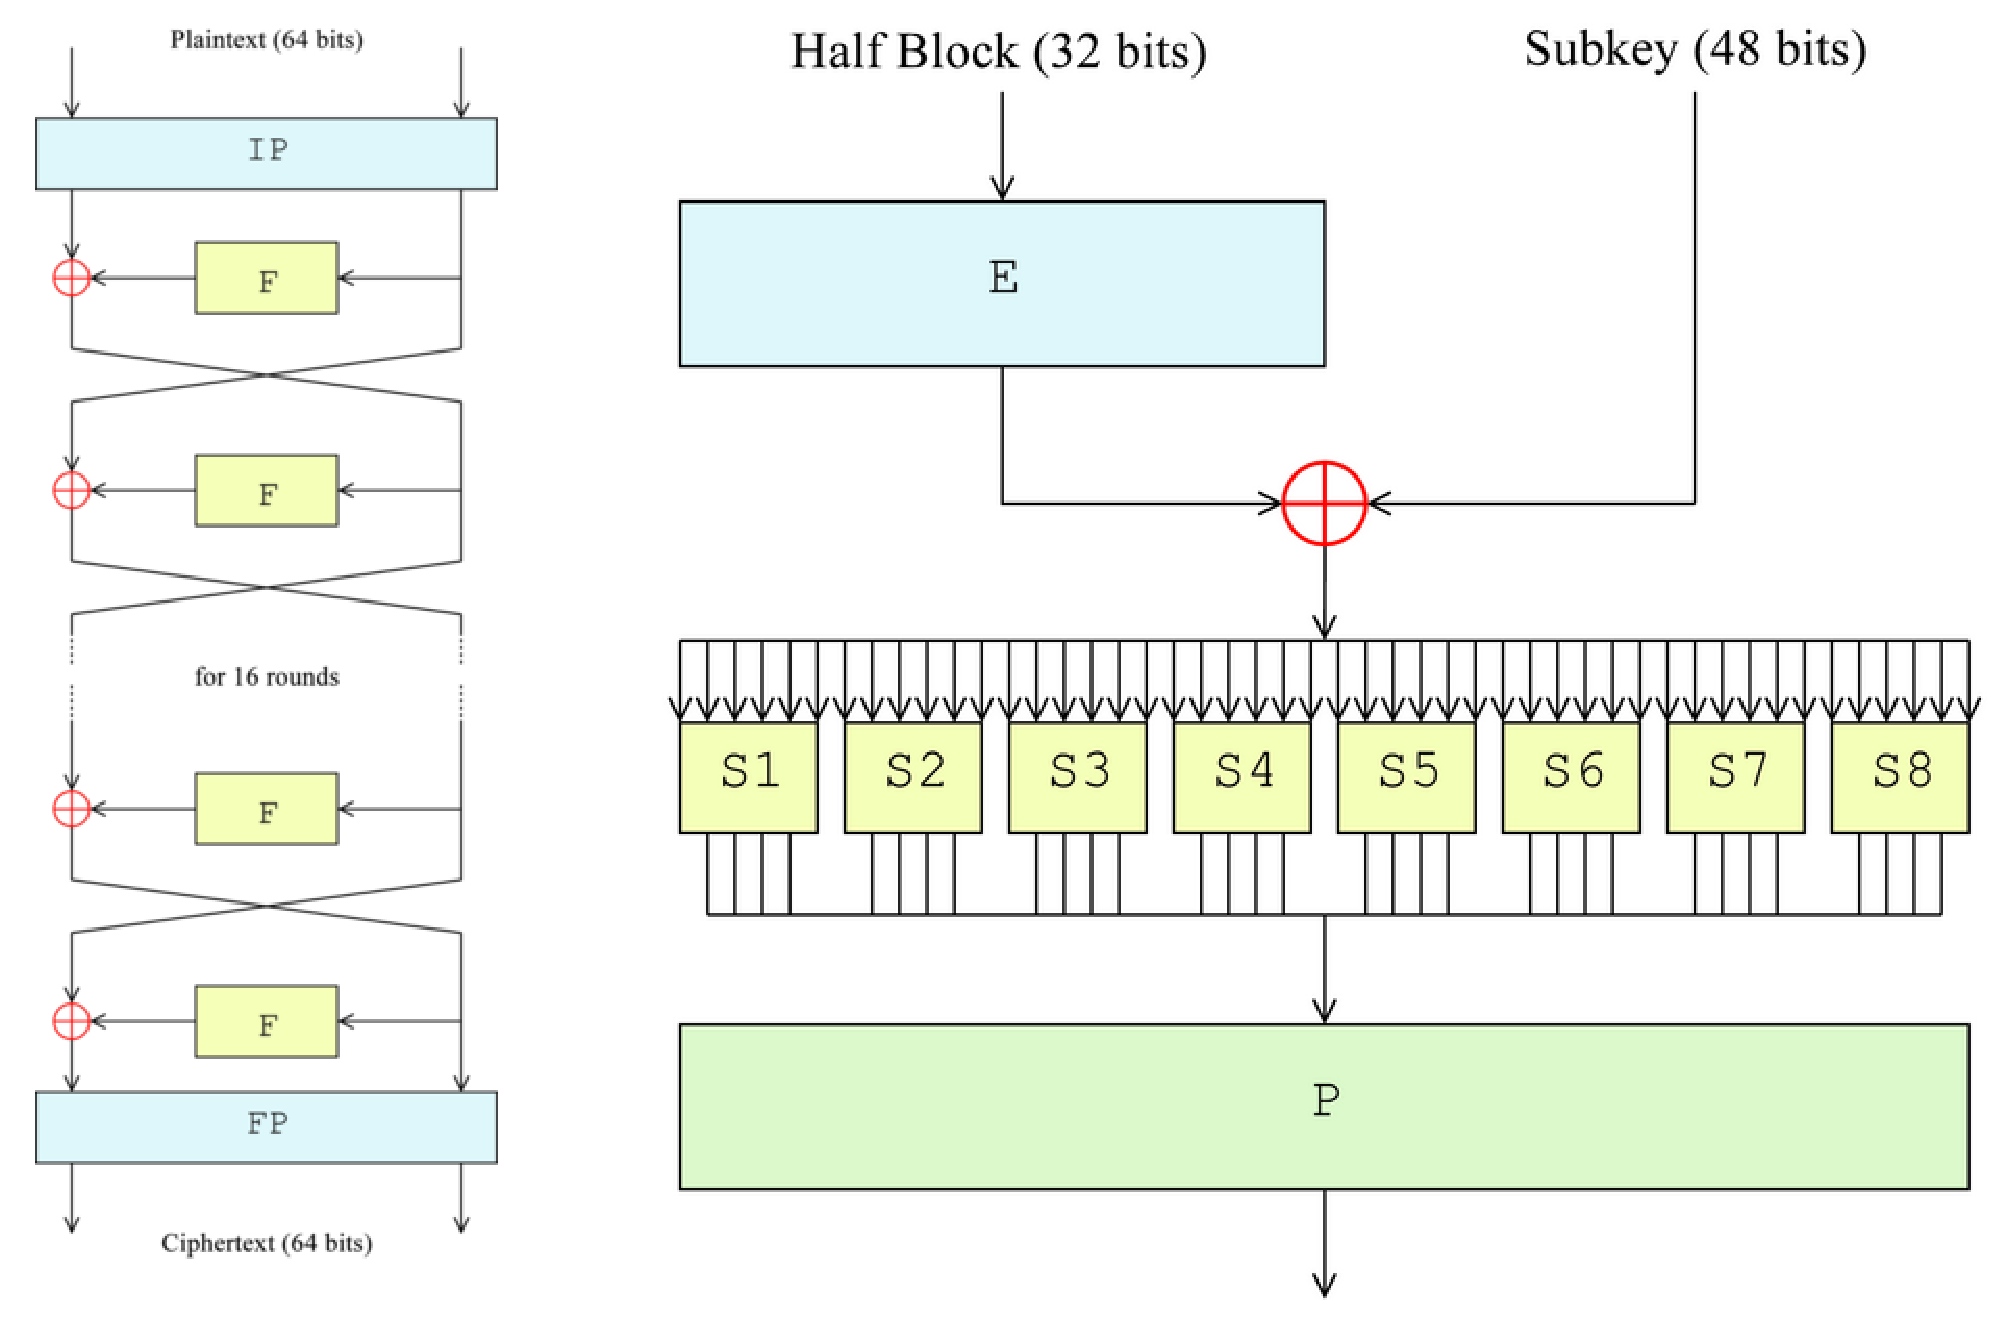
\includegraphics[scale=0.4]{pics/DES.eps}
 \end{center}

\subsection{How does encryption work?}
Different approaches:
\begin{itemize}
	\item public key cryptography (example: {\em RSA})
		\begin{itemize}
			\item Paula has a private and a public key
			\item data encrypted with her private key can only be decrypted by
				her public key and vice versa
			\item public key can be shared with David
		\end{itemize}
\end{itemize}

\begin{center}
	\includegraphics[scale=0.4]{pics/Public_key_encryption.eps}
 \end{center}

\subsection{Accuracy or Integrity}
In order to protect against forgery or data manipulation, provide some sort of
digest or checksum (often a one-way hash).  Popular choices:

\begin{itemize}
	\item {\tt 5f4dcc3b5aa765d61d8327deb882cf99}
	\item {\tt 5baa61e4c9b93f3f0682250b6cf8331b7ee68fd8}
	\item {\tt 5e884898da28047151d0e56f8dc6292773603d0d6aabbdd62 \
                   a11ef721d1542d8}
	\item {\tt b109f3bbbc244eb82441917ed06d618b9008dd09b3befd1b5 \
                   e07394c706a8bb980b1d7785e5976ec049b46df5f1326af5a \
                   2ea6d103fd07c95385ffab0cacbc86}
\end{itemize}

\subsection{Accuracy or Integrity}
In order to protect against forgery or data manipulation, provide some sort of
digest or checksum (often a one-way hash).  Popular choices:

\begin{itemize}
	\item {\tt 5f4dcc3b5aa765d61d8327deb882cf99} (MD5)
	\item {\tt 5baa61e4c9b93f3f0682250b6cf8331b7ee68fd8} (SHA-1)
	\item {\tt 5e884898da28047151d0e56f8dc6292773603d0d6aabbdd62 \
                   a11ef721d1542d8} (SHA256)
	\item {\tt b109f3bbbc244eb82441917ed06d618b9008dd09b3befd1b5 \
                   e07394c706a8bb980b1d7785e5976ec049b46df5f1326af5a \
                   2ea6d103fd07c95385ffab0cacbc86} (SHA512)
\end{itemize}

\subsection{Accuracy or Integrity}
In order to protect against forgery or data manipulation, provide some sort of
digest or checksum (often a one-way hash).  Popular choices:

\begin{itemize}
	\item {\tt 5f4dcc3b5aa765d61d8327deb882cf99} (MD5)
	\item {\tt 5baa61e4c9b93f3f0682250b6cf8331b7ee68fd8} (SHA-1)
	\item {\tt 5e884898da28047151d0e56f8dc6292773603d0d6aabbdd62 \
                   a11ef721d1542d8} (SHA256)
	\item {\tt b109f3bbbc244eb82441917ed06d618b9008dd09b3befd1b5 \
                   e07394c706a8bb980b1d7785e5976ec049b46df5f1326af5a \
                   2ea6d103fd07c95385ffab0cacbc86} (SHA512)
\end{itemize}


Caveats:
\begin{itemize}
	\item ``rainbow tables'' / internet search engines allow for easy reverse
		lookup of un-salted hashes.
	\item integrity only ensured if authenticity of information itself is
		guaranteed
\end{itemize}

%\subsection{Authenticity}
%\begin{figure}[hb]
%    \begin{center}
%        \includegraphics[scale=0.63]{sniff.eps} \\
%    \end{center}
%\end{figure}
%
\subsection{Authenticity}
\begin{itemize}
	\item in private key cryptography, authenticity is (often) assumed/implied
	\item in public key cryptography, often accomplished via a separate
		signature
	\item ways to establish assurance of authenticity for parties that have
		never met:
		\begin{itemize}
			\item public key infrastructures (PKI) and certificate
				authorities (CA)
			\item ``web of trust''
		\end{itemize}
\end{itemize}


\subsection{Authentication}
First, the client needs to prove that it knows the secret.  This is done in
the encryption handshake, consisting of a {\em challenge} and a {\em
response}.
\vspace{.125in}
\begin{figure}[hb]
    \begin{center}
        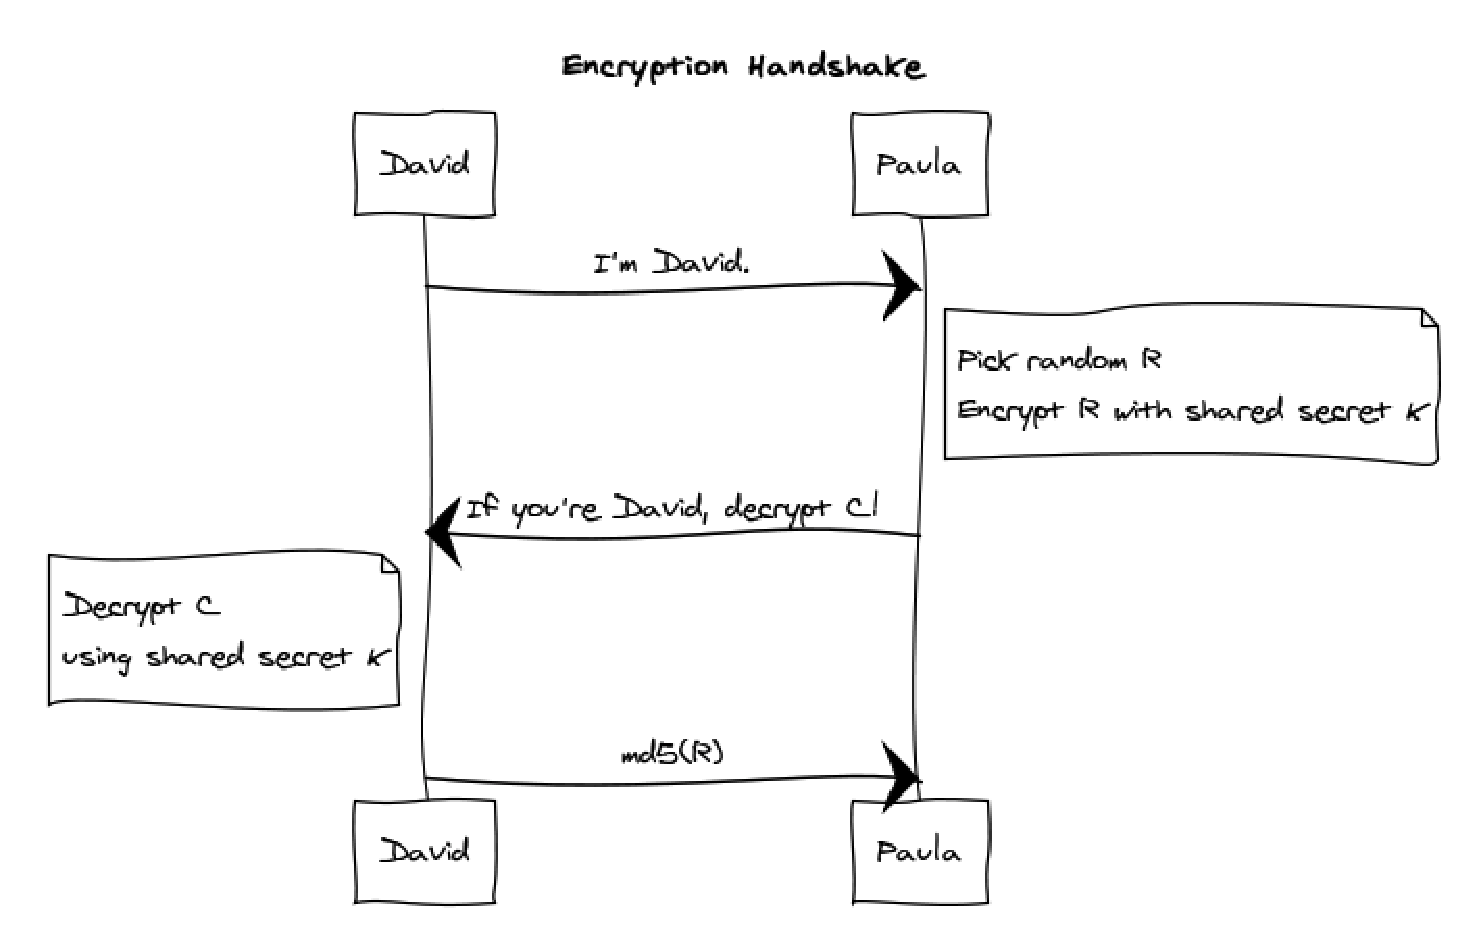
\includegraphics[scale=0.65]{pics/handshake2.eps} \\
    \end{center}
\end{figure}

\subsection{Random String generation}
Random numbers can be generated using {\tt /dev/random}, {\tt
/dev/urandom}, {\tt rand(3)}, {\tt random(3)}, {\tt openssl\_bn(3)} etc.
\\

Map numbers to printable characters (for example, see {\tt
http://is.gd/G55X5R}):

\begin{verbatim}
static const unsigned char itoa64[] =
        "./0123456789ABCDEFGHIJKLMNOPQRSTUVWXYZabcdefghijklmnopqrstuvwxyz";

char salt[16];
for (i=0; i<16; i++)
        salt[i] = itoa64[(int)random()%64];

\end{verbatim}

\subsection{Random String generation}
Random numbers can be generated using {\tt /dev/random}, {\tt
/dev/urandom}, {\tt rand(3)}, {\tt random(3)}, {\tt openssl\_bn(3)} etc.
\\

Map numbers to printable characters using ASCII values:

\begin{verbatim}
for (i=0; i<16; i++) {
        int c = 0;

        while(c < 32 || c > 255)
                c = (int)arc4random()%255;
        salt[i] = c;
}
\end{verbatim}


\subsection{Blowfish}
See {\tt blowfish(3)}:
\begin{itemize}
	\item a symmetric block cipher
	\item variable key length (we'll use 128 bit)
	\item consists of a key setup phase and the actual encryption or
		decryption
	\item use of {\tt ivec}, which needs to be shared
\end{itemize}

\subsection{Electronic Codebook Mode}
\begin{figure}[hb]
    \begin{center}
        \includegraphics{pics/Ecb_encryption.eps} \\
    \end{center}
\end{figure}

\subsection{Electronic Codebook Mode}
\begin{figure}[hb]
    \begin{center}
        \includegraphics{pics/Ecb_decryption.eps} \\
    \end{center}
\end{figure}

\subsection{Cipher Block Chaining}
\begin{figure}[hb]
    \begin{center}
        \includegraphics{pics/Cbc_encryption.eps} \\
    \end{center}
\end{figure}

\subsection{Cipher Block Chaining}
\begin{figure}[hb]
    \begin{center}
        \includegraphics{pics/Cbc_decryption.eps} \\
    \end{center}
\end{figure}

\subsection{Sharing a per-session {\tt ivec}}
\begin{figure}[hb]
    \begin{center}
        \includegraphics[scale=0.52]{pics/ivec.eps} \\
    \end{center}
\end{figure}

\subsection{HW\#5}
\verb+http://www.cs.stevens.edu/~jschauma/631/f11-hw5.html+

Verify your code works:
\begin{verbatim}
$ cat input | openssl bf-cbc -K cafefacedeadbeef -iv 0 > secret
$ ./bfed -d -k cafefacedeadbeef <secret >output
$ diff input output

$ cat input | ./bfed -e -k cafefacedeadbeef > secret
$ cat secret | openssl bf-cbc -d -K cafefacedeadbeef -iv 0 > output
$ diff input output

\end{verbatim}


\subsection{References}
OpenSSL's crypto libraries:
\begin{itemize}
	\item {\tt crypto(3)}, {\tt blowfish(3)}
	\item {\tt EVP\_EncryptInit(3)}
%	\item {\tt http://tldp.org/LDP/LG/issue87/vinayak.html}
	\item {\tt http://en.wikipedia.org/wiki/Cipher\_Block\_Chaining}
\end{itemize}

\end{document}
